\documentclass[11pt,a4paper,oneside]{article}
\usepackage[dutch]{babel}
\usepackage{amsmath}
\usepackage{graphicx}
\usepackage{tikz}
\usepackage{fancyhdr}
\usepackage{dsfont}
\usepackage{parskip}
\usepackage{epstopdf}
\usepackage{listings}
\usepackage{color}
\definecolor{lichtgrijs}{gray}{0.95}
\usepackage{cite}
\usepackage[nottoc]{tocbibind}
\usepackage[T1]{fontenc}
\usepackage[light,math]{iwona}
\usepackage{pgfplots}
%\pgfplotsset{compat=newest}
\usepackage{subfig}
\usepackage{textcomp}
\usetikzlibrary{arrows,automata}
\usepackage{float}
\usepackage{longtable}
\usepackage{titling,enumitem}
\usepackage{a4wide}
\usepackage{amssymb}
\usepackage{rotating}
\usepackage{listings}
\usepackage[top=1.1in, bottom=1.2in, left=1.1in, right=1.1in]{geometry}
\usepackage{array}
\usepackage{titling}
\usepackage{blindtext}
\usepackage{chngpage}
\usepackage{calc}
\definecolor{lightgray}{gray}{0.8}
\newcolumntype{L}{>{\raggedleft}p{0.50\textwidth}}
\newcolumntype{R}{p{0.8\textwidth}}
\newcommand\VRule{\color{lightgray}\vrule width 0.5pt}
\usepackage{color, colortbl}
\definecolor{Gray}{gray}{0.9}
\definecolor{dkgreen}{rgb}{0,0.6,0}
\definecolor{gray}{rgb}{0.5,0.5,0.5}
\definecolor{mauve}{rgb}{0.58,0,0.82}
\definecolor{ugentblue}{rgb}{0.05,0.18,0.37}
\usepackage{import}
\usepackage[T1]{fontenc}
\begin{document}

%\newgeometry{top=0.8cm, right=1.70cm, left=1.7cm}
\begin{titlepage}

\thispagestyle{fancy}
\fancyhf{}
\fancyfoot[L]{}
\begin{figure}[!ht]
  \begin{adjustwidth}{-\oddsidemargin-1in}{-\rightmargin}
    \centering
    
\includegraphics[width=\paperwidth]{banner}
  \end{adjustwidth}
\end{figure}
\vspace{-0.2em}
\begin{center}
\vspace{5cm}
\Huge \textbf{Vakoverschrijdend Project: team Edran\\ Rapport episode 2}\\
\vspace{6.0cm}
\large
\begin{tabular}{L! {} R}
& {\LARGE\bf Team Edran} \\
& \\
& {\bf Steven De Blieck} \\
& {\bf Laurens De Graeve} \\
& {\bf Bart Middag} \\
& {\bf Wouter Pinnoo} \\
& {\bf Robin Praet} \\
& {\bf Stijn Seghers} \\
& {\bf Wouter Termont} \\
& {\bf Gilles Vandewiele} \\
\end{tabular}
\end{center}
\end{titlepage}
%\restoregeometry
\newpage

\fancyheadoffset[RO,LE]{0in}
\fancypagestyle{plain}{
\fancyhead[L]{Rapport episode 2}
\fancyhead[R]{Team Edran}
\fancyfoot[L]{}
\fancyfoot[R]{\thepage}}

\fancyhead[L]{Rapport episode 2}
\fancyhead[R]{Team Edran}
\fancyfoot[L]{}
\fancyfoot[C]{\thepage}
\pagestyle{fancy}
\tableofcontents
\newpage

\setcounter{section}{0}
\setcounter{subsection}{0}
\part{Verwachte functionaliteiten}
\begin{itemize}
	\item	Een autolener/eigenaar moet zich kunnen registreren in het systeem.
		\begin{itemize}
			\item	Om wachtwoorden en andere gevoelige informatie op te slaan, zal een encryptiemechanisme gebruikt worden.
		\end{itemize}
	\item	Een gereserveerde gebruiker moet zich hierna ook kunnen inloggen in het systeem.
	\item	Ieder soort gebruiker komt overeen met een bepaalde rol. De pagina reageert anders op een gebruiker van een bepaalde rol, dan van een andere (bijvoorbeeld: enkel een admin kan het tabblad beheer zien).
	\item	Nadat een gebruiker een rit gemaakt heeft, moet hij hierover ritgegevens kunnen invullen.
	\item	Deze ritgegevens moeten goed- of afgekeurd worden door de autoeigenaar.
	\item	Aan de hand van alle ingevoerde, goedgekeurde ritgegevens kan door een admin een factuur opgesteld worden voor alle gebruikers van het systeem. Ook moeten de prijzen makkelijk aangepast kunnen worden.
	\item	Om vlugger en gebruiksvriendelijker te kunnen reserveren, implementeren we een filtersysteem bij de kalender.
\end{itemize}

\setcounter{section}{0}
\setcounter{subsection}{0}
\part{Registratie en inloggen}
\section{Usecases}
\subsection{Een nieuwe autolener registreert zich}
Een nieuwe gebruiker kan zich registreren door naar de pagina "registreren als autolener" te gaan op de website. Hierbij moet hij zijn naam, voornaam, adres, postcode, stad, telefoonnummer ingeven en zijn wachtwoord en email twee keer. Hierna kan de gebruiker zich optioneel registreren voor een infosessie. \\
Hierna controleert het systeem of het gegeven emailadres uniek is en slaat alle nodige informatie van de gebruiker op in de databank. Hierbij wordt het wachtwoord eerst ge\"{e}ncrypteerd. Er wordt ook een email naar de gebruiker gestuurd met zijn inloginformatie (meegegeven email en wachtwoord).

\subsection{Een nieuwe autoeigenaar registreert zich}
De registratie van een autoeigenaar is uitgebreider dan die van een autolener. Een autoeigenaar doorloopt dezelfde procedure als die van een autolener, behalve dat de infosessies aangepast zijn voor autoeigenaars. Hierbovenop moet de gebruiker ook informatie over de te registreren auto ingeven: automerk, model, bouwjaar, brandstof, jaarlijkse kilometers, huidige kilometerstand, naam verzekering, vervaldatum polis, polisnummer, bonus-malus, aantal zitplaatsen, trekhaak, GPS, gemiddelde verbruik per kilometer, huidige geschatte waarde, nummerplaat, volume koffer, inschrijvingsbewijs, chassisnummer en verschillende foto's van de verschillende aanzichten van de auto. Hierbovenop kan er ook nog optioneel commentaar toegevoegd worden. \\
Nu wordt opnieuw de uniciteit van het emailadres gecontroleerd, de informatie wordt opgeslagen in de databank en een email wordt naar de gebruiker gestuurd.

\subsection{Een gebruiker logt in op het systeem}
Om in te loggen op het systeem moet de gebruiker naar de pagina 'Inloggen' op de webpagina gaan. Hier geeft hij zijn email en wachtwoord in, die door het systeem gevalideerd worden. Naargelang de gebruiker een nieuw geregistreerde gebruiker, autolener, admin of autobeheerder is, toont het systeem nu een nieuwe interface voor de gebruiker. Iedere gebruiker krijgt 'Notificaties' en 'Mijn gegevens' te zien. 
\begin{itemize}
	\item	Een nieuw geregistreerde gebruiker die nog niet naar een infosessie is geweest, krijgt enkel het tabblad 'Infosessies' te zien, waar hij zich kan inschrijven voor een infosessie
	\item	Indien de gebruiker reeds naar een infosessie is geweest, maar zijn registratie nog niet vervolledigt heeft, ziet de gebruiker geen enkel tabblad zolang de nodige informatie nog niet doorgegeven is. (zie registratie vervolledigen)
	\item	Indien een autolener is ingelogd, krijgt deze enkel het tabblad 'Lenen te zien'
	\item	Indien een eigenaar is ingelogd, krijgt hij het tabblad 'Lenen' en 'Autobeheer' te zien.
	\item	Indien een admin is ingelogd, krijgt hij het tabblad 'Beheer' te zien.
\end{itemize}

\subsection{Een gebruiker vervolledigt zijn registratie}
Wanneer een gebruiker naar een infosessie is geweest, moet hij nog extra informatie doorgeven: domicilie- en verblijfsadres, rijksregisternummer, identiteitskaartnummer (en een scan hiervan), een scan van zijn rijbewijs en een schadeverleden. Hierbovenop moet de gebruiker ook nog akkoord gaan met de algemene voorwaarden (die op de infosessie uitgelegd zijn). Het systeem slaat alle nodige informatie op en brengt alle admins op de hoogte, deze moeten deze informatie hierna goedkeuren. Als de volledige procedure is doorlopen, is de geregistreerde gebruiker nu een volwaardige gebruiker van het systeem.

\subsection{Een beheerder keurt een registratie goed}
Als een beheerder de machtiging heeft om registraties goed/af te keuren, kan hij hiervoor naar een aparte pagina gaan. Hier krijgt hij een lijst met alle registraties die nog in aanvraag zijn. Van iedere registratie kan hij de meegeven informatie bekijken om dan de registratie goed of af te keuren. Indien de registratie goedgekeurd wordt, zal de gebruiker een volwaardig lid worden. Indien de registratie afgekeurd wordt, zal de gebruiker hiervan op de hoogte gebracht worden aan de hand van een email.

\subsection{Een gebruiker vraagt zijn wachtwoord opnieuw op}
Indien de gebruiker zijn wachtwoord vergeten is, kan hij dit opnieuw opvragen. Hierbij geeft hij zijn emailadres in, waarna het systeem een email zal sturen naar de gebruiker met daarin een link om zijn wachtwoord te resetten. Als de gebruiker binnen de 24 uur op deze link klikt, krijgt hij een nieuw wachtwoord toegewezen.

\section{Mockups}
\subsection{Inloggen}
\begin{figure}[H]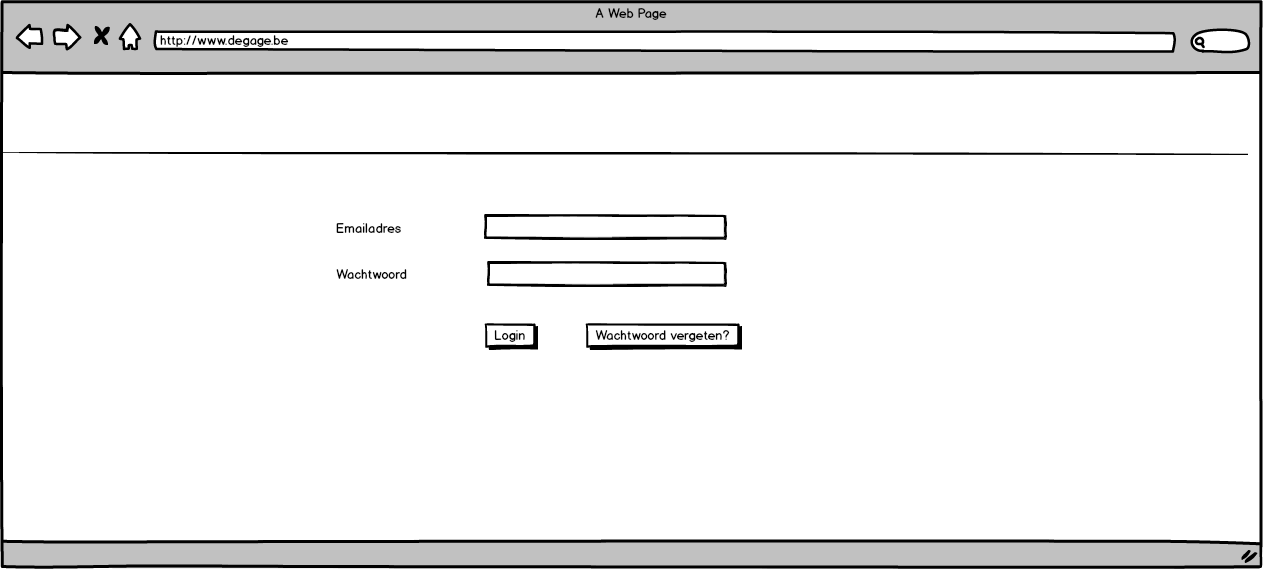
\includegraphics[width=\textwidth]{../../mockups/login.png}\end{figure}

\subsection{Registreren als autolener}
\begin{figure}[H]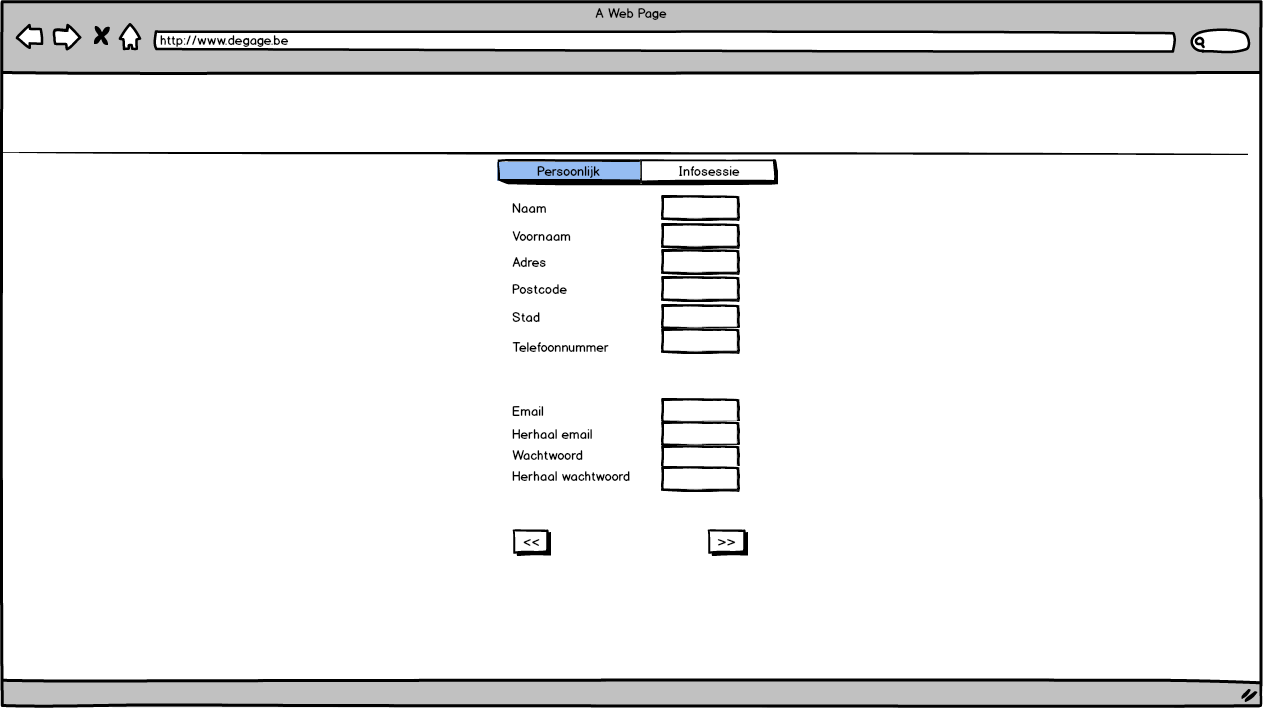
\includegraphics[width=\textwidth]{../../mockups/registratie_autolener_persoonlijk.png}\end{figure}
\begin{figure}[H]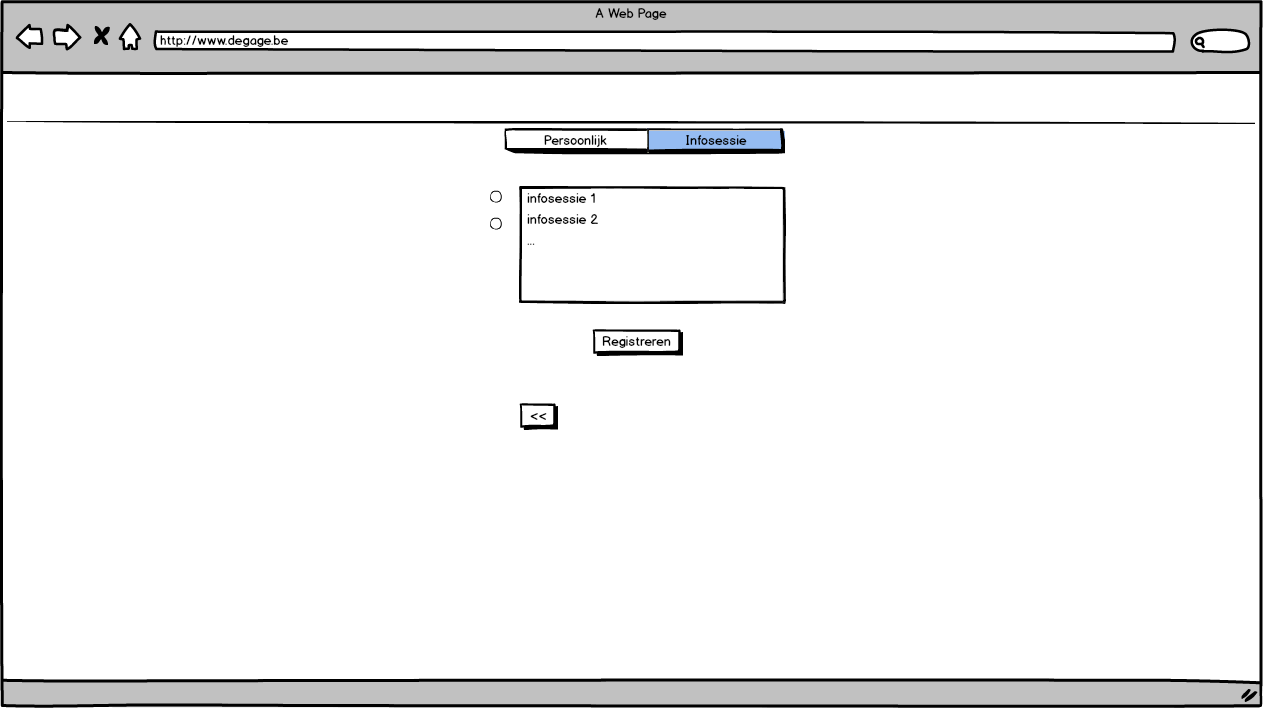
\includegraphics[width=\textwidth]{../../mockups/registratie_autolener_infosessie.png}\end{figure}

\subsection{Registreren als autoeigenaar}
\begin{figure}[H]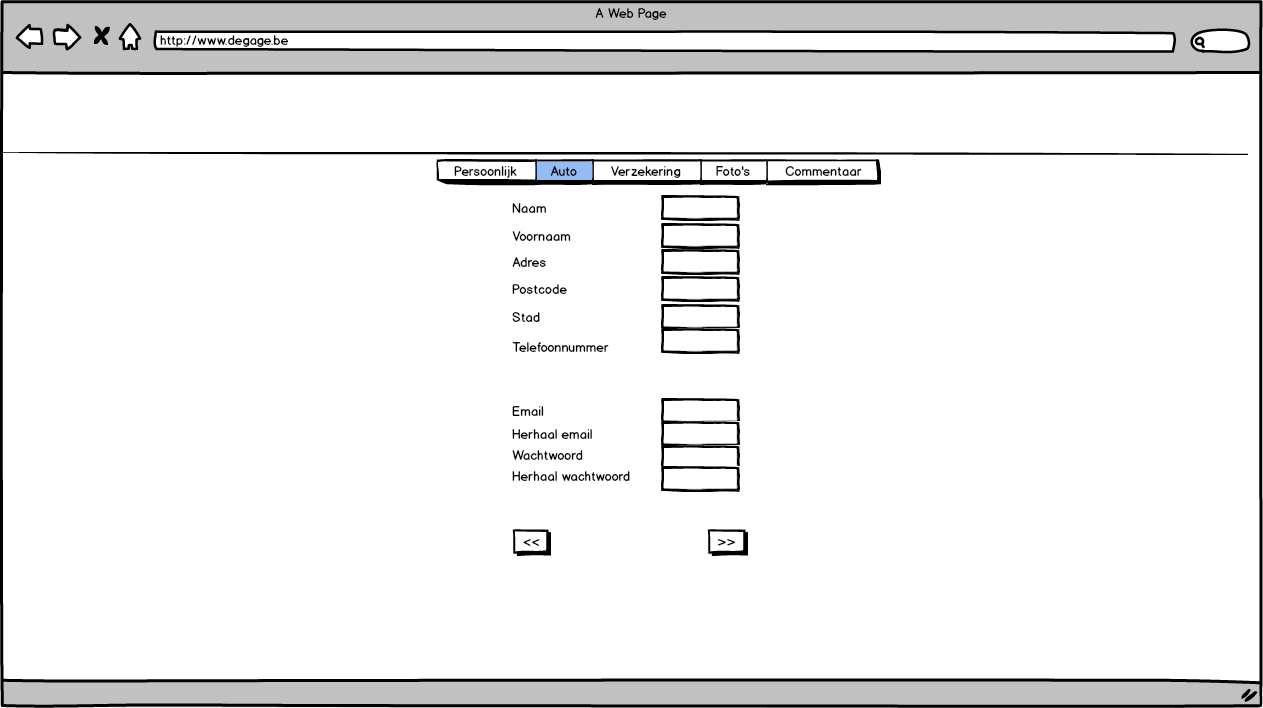
\includegraphics[width=\textwidth]{../../mockups/registratie_eigenaar_persoonlijk.png}\end{figure}
\begin{figure}[H]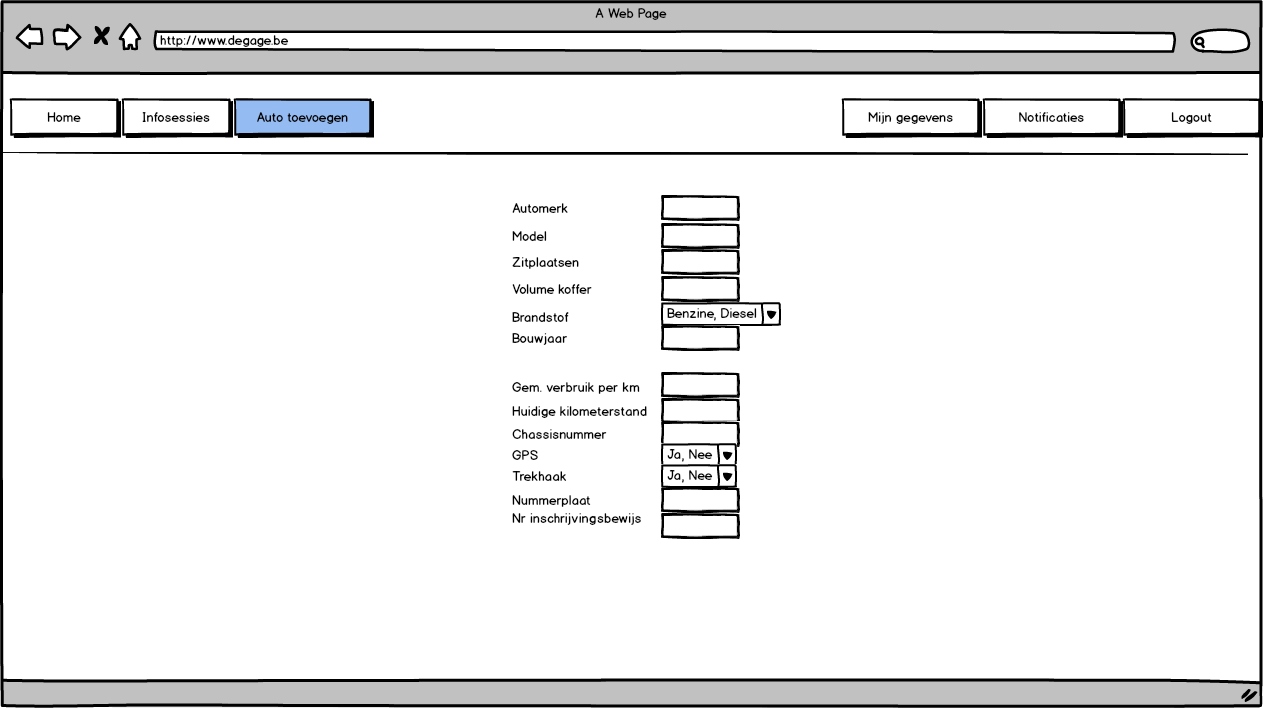
\includegraphics[width=\textwidth]{../../mockups/registratie_eigenaar_auto.png}\end{figure}
\begin{figure}[H]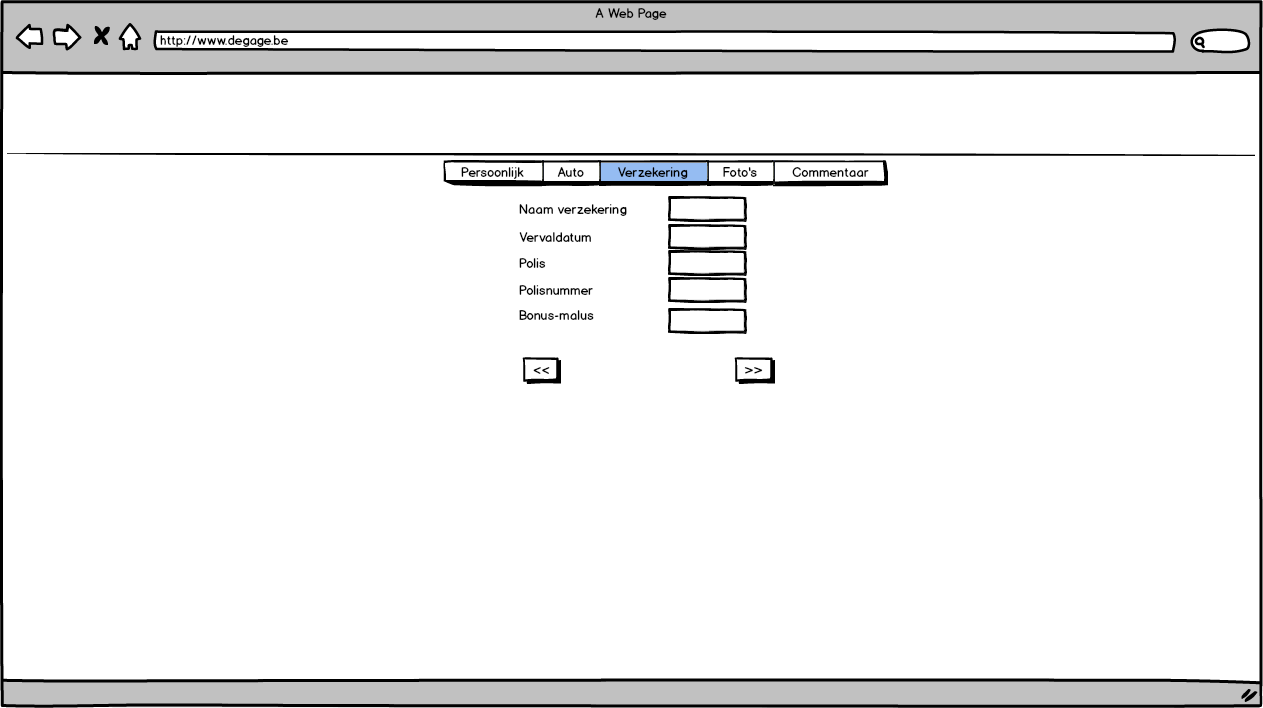
\includegraphics[width=\textwidth]{../../mockups/registratie_eigenaar_verzekering.png}\end{figure}
\begin{figure}[H]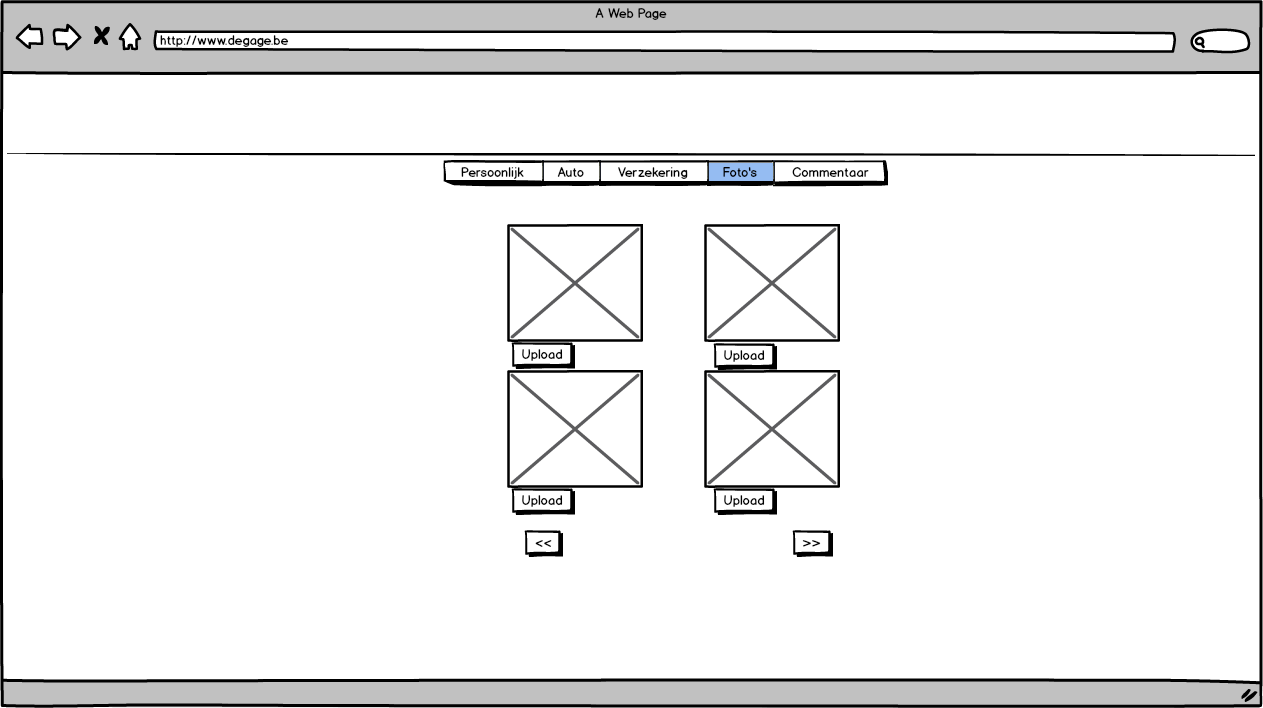
\includegraphics[width=\textwidth]{../../mockups/registratie_eigenaar_fotos.png}\end{figure}
\begin{figure}[H]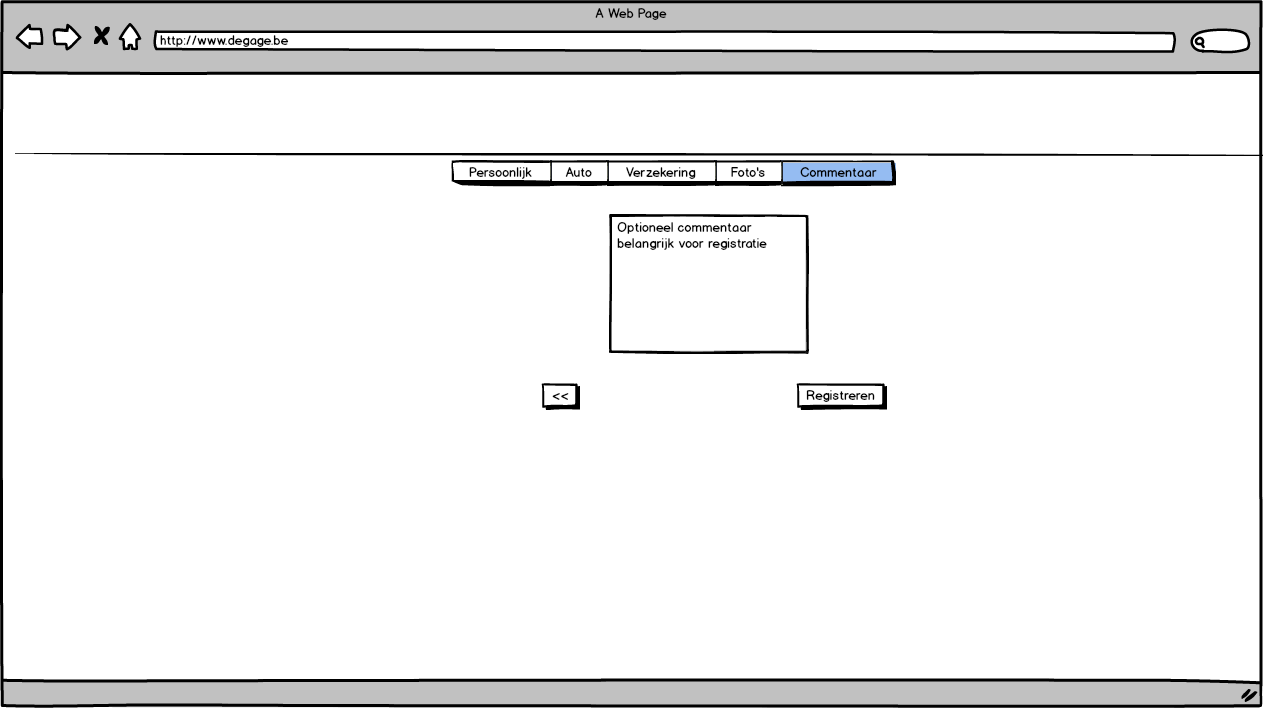
\includegraphics[width=\textwidth]{../../mockups/registratie_eigenaar_commentaar.png}\end{figure}

\subsection{Registratie vervolledigen}
\begin{figure}[H]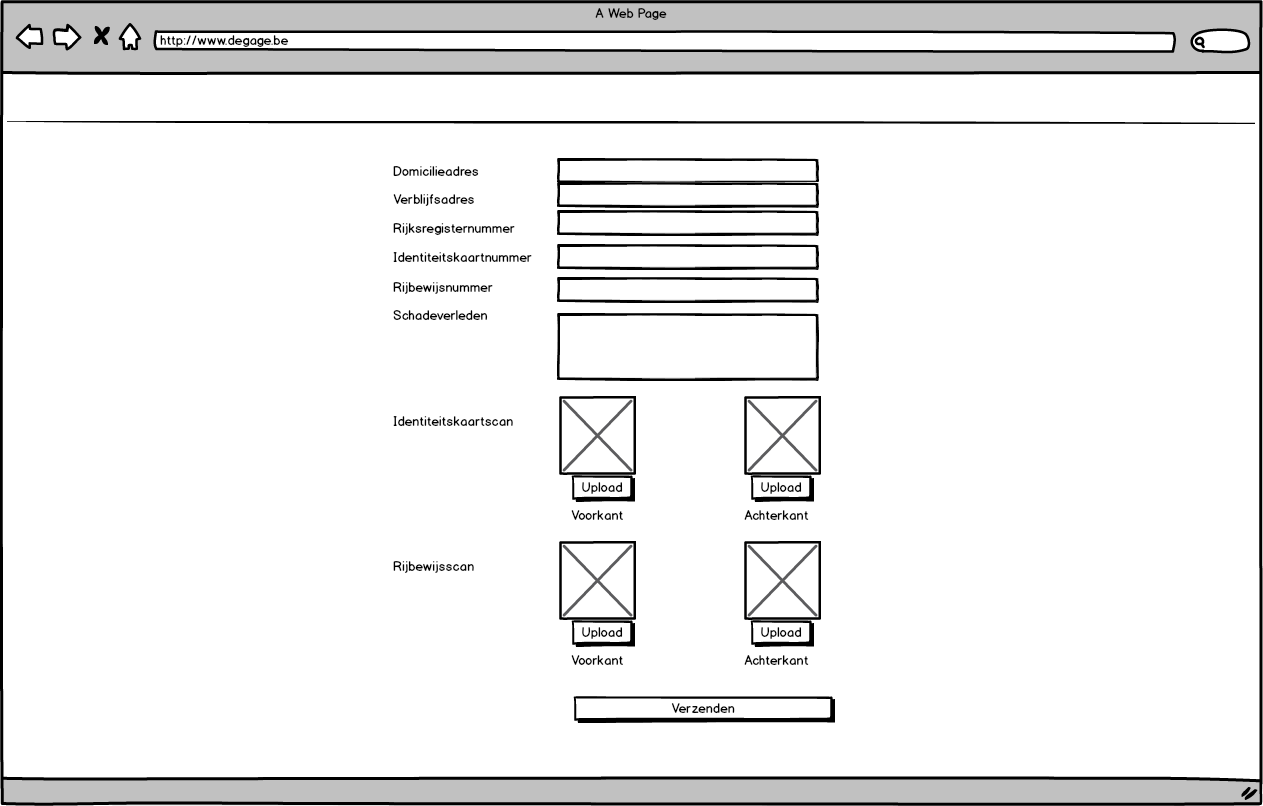
\includegraphics[width=\textwidth]{../../mockups/registratievervolledigen.png}\end{figure}

\subsection{Wachtwoord vergeten}
\begin{figure}[H]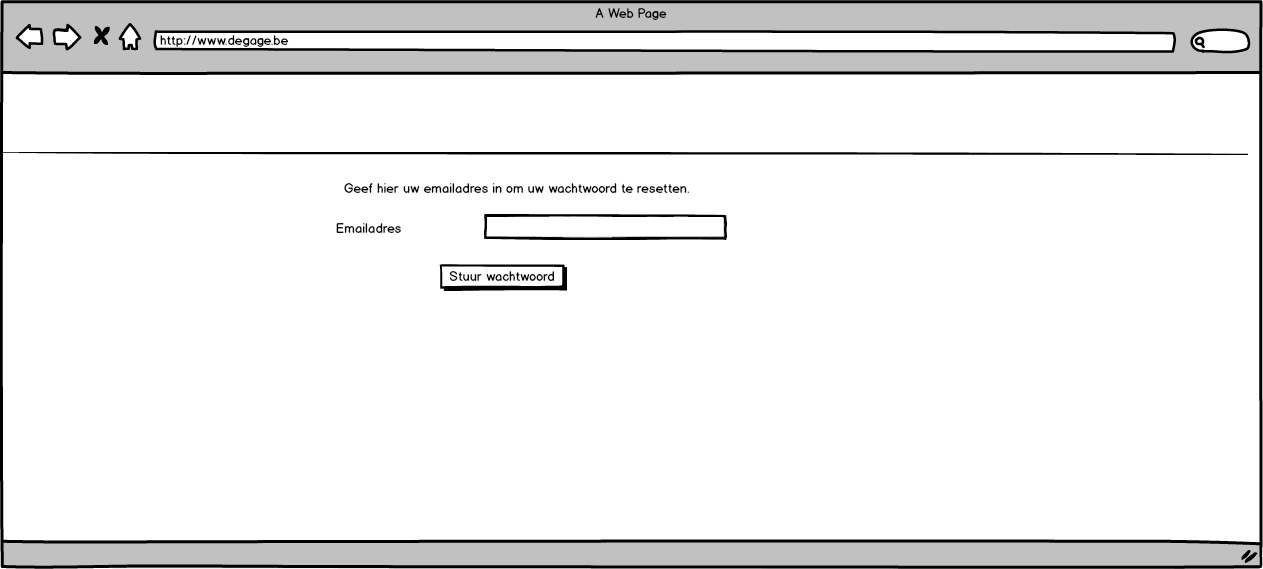
\includegraphics[width=\textwidth]{../../mockups/wachtwoordvergeten.png}\end{figure}

\setcounter{section}{0}
\setcounter{subsection}{0}
\part{Doorgeven, goedkeuren en afkeuren van ritgegevens}

\section{Usecases}
\subsection{Ritgegevens inbrengen}
Nadat een autolener met een auto gereden heeft, moet hij ritgegevens van de rit inbrengen. Dit zijn onder meer de nieuwe kilometerstand, of er al dan niet getankt is en andere soorten bewijsmateriaal (zoals bijvoorbeeld een carwash). Dit kan de gebruiker doen op een apart tabblad "Ritgegevens" onder de pagina "Lenen". Indien er ook schade opgelopen is, moet een admin gecontacteerd worden. Nadat alle gegevens ingevoerd zijn, worden deze in de databank opgeslagen en wordt er een notificatie naar de autoeigenaar, van de auto waarmee de rit is gemaakt, gestuurd.

\subsection{Ritgegevens goed- of afkeuren}
Onder het tabblad "Autobeheer" kan de autoeigenaar ritgegevens over ritten met zijn auto goed- of afkeuren. Hiervoor selecteert hij de gewenste ritgegevens in een tabel en klikt hierna op accepteren of weigeren. Indien de ritgegevens geweigerd worden moet er een reden meegegeven worden en de gegevens opnieuw door de gebruiker ingevoerd worden. Ritgegevens van een autoeigenaar moeten door een beheerder goedgekeurd worden.


\section{Mockups}
\subsection{Doorgeven van ritgegevens}
\begin{figure}[H]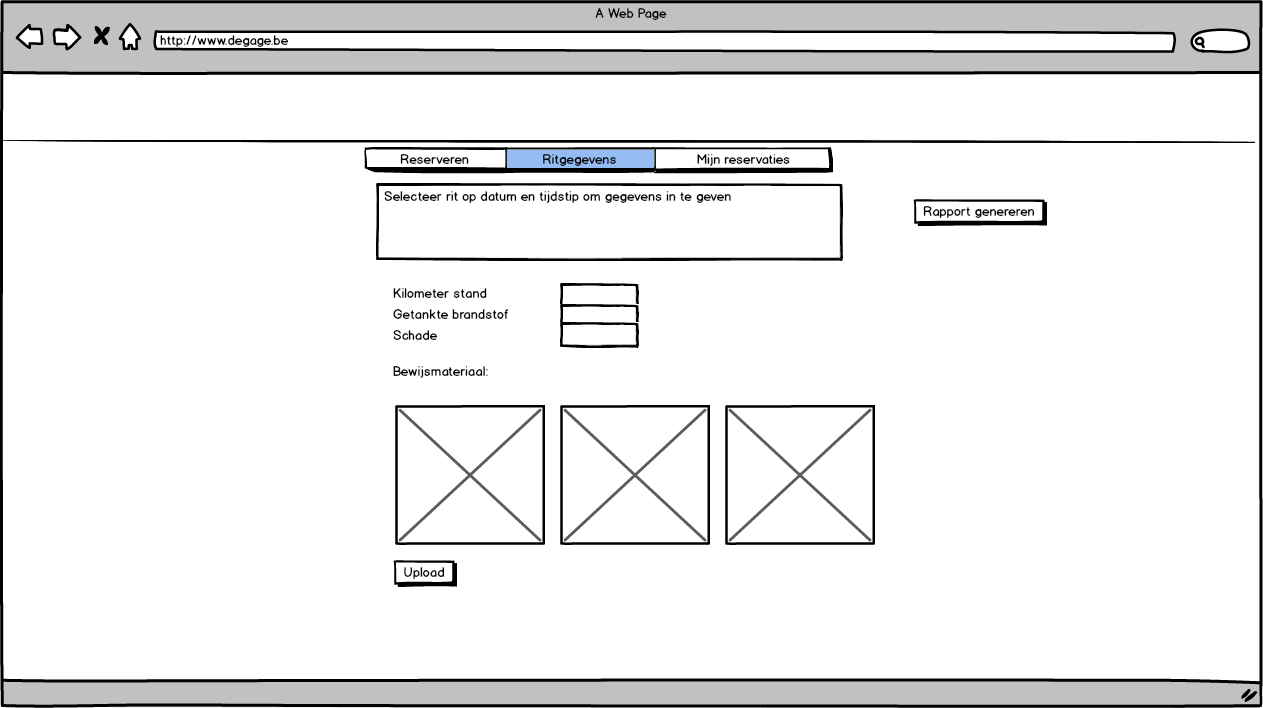
\includegraphics[width=\textwidth]{../../mockups/delen_ritgegevens.png}\end{figure}

\subsection{Goed- en afkeuren van ritgegevens}
\begin{figure}[H]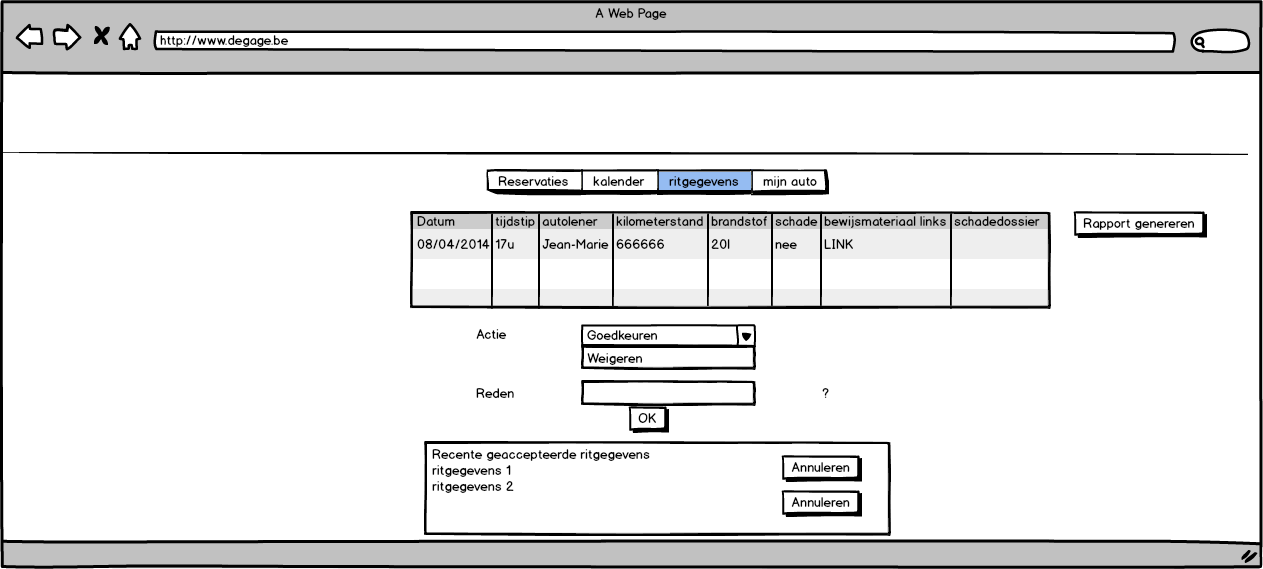
\includegraphics[width=\textwidth]{../../mockups/autobeheer_ritgegevens.png}\end{figure}

\setcounter{section}{0}
\setcounter{subsection}{0}
\part{Facturisatie + beheer}

\section{Usecases}
\subsection{Aanpassen van de parameters horende bij de facturisatie}
Op de beheerspagina kan de beheerder de prijscategorie\"{e}n, de intervallen en de prijs per categorie aanpassen.

\subsection{Afrekening maken}
Wanneer de admin op een knop klikt op de pagina "Beheer", wordt er voor alle gebruikers een factuur opgesteld. Deze facturen kunnen hierna gecontroleerd worden en automatisch gemaild worden naar de gebruikers. De kostprijs wordt gemaakt aan de hand van de gemaakte ritten (waarvan de doorgegevens ritgegevens ook goedgekeurd zijn). Hier worden optioneel nog de zelf gemaakte kosten van af getrokken. Voor een autoeigenaar moeten de ritgegevens door een beheerder goedgekeurd worden, en kan het geval zich voordoen dat er een factuur van D\"{e}gage moet opgemaakt worden, in plaats van voor de eigenaar (indien de kosten gemaakt met zijn auto groter zijn dan de kosten gemaakt door zichzelf).

\section{Mockups}
\subsection{Beheer van de prijzen voor facturisatie}
\begin{figure}[H]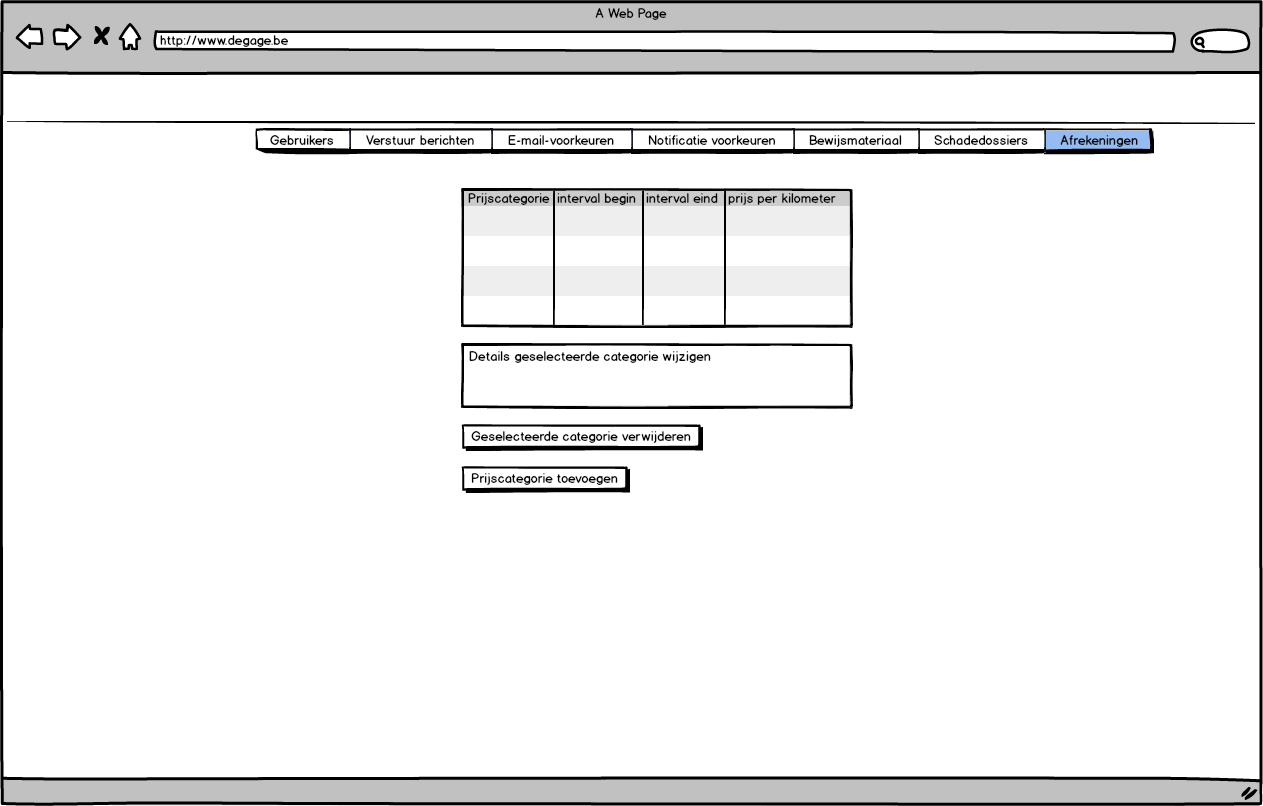
\includegraphics[width=\textwidth]{../../mockups/admin_afrekening_voorkeuren.png}\end{figure}
\subsection{Afrekening maken}
\begin{figure}[H]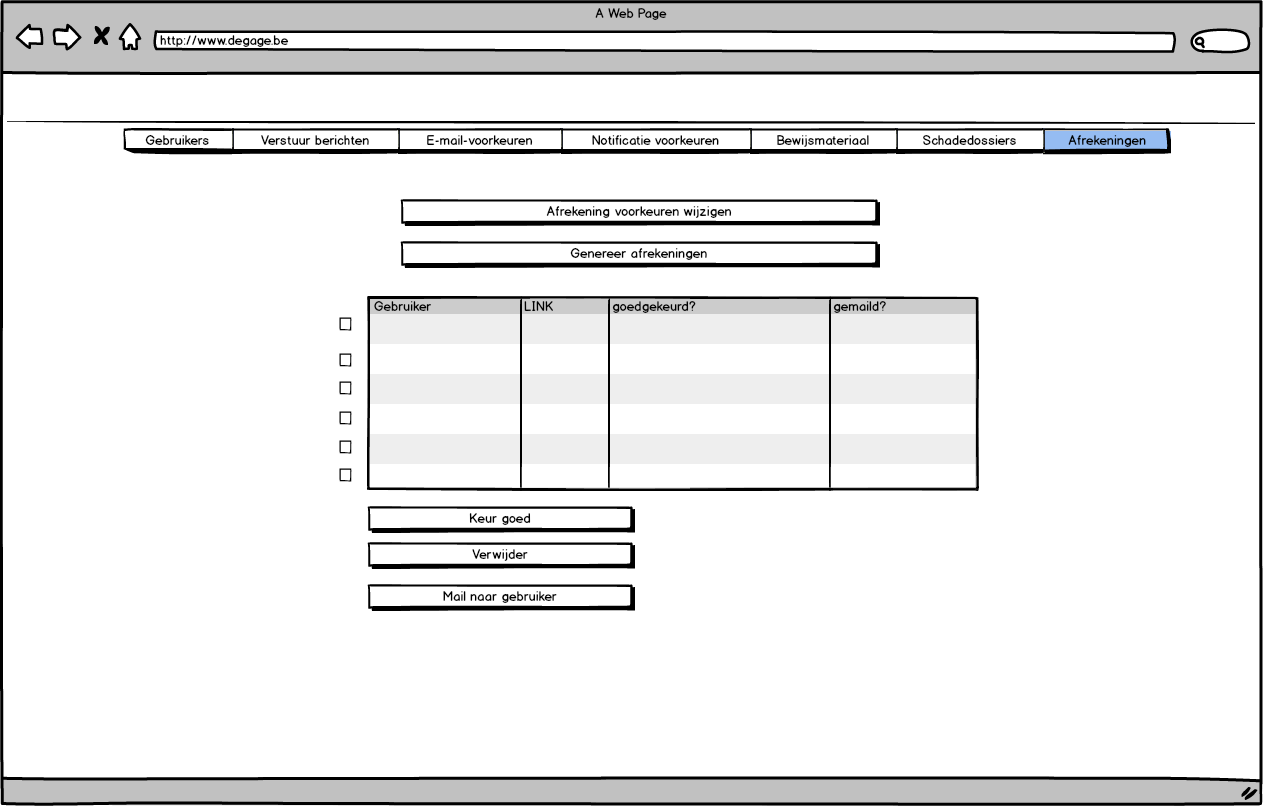
\includegraphics[width=\textwidth]{../../mockups/admin_afrekeningen.png}\end{figure}
\setcounter{section}{0}
\setcounter{subsection}{0}
\part{Filtersysteem bij kalender}
\section{Usecases}
\subsection{Filteren van de kalender op basis van parameters}
Een autolener kan bij het reserveren eerst en vooral een bepaalde datum kiezen. Daarna kan hij een startuur en einduur opgeven om beschikbare auto's weer te geven. Er kan ook verder gespecificeerd worden. De autolener kan de duur van de gewenste leenperiode in dagen en uren uitdrukken. Via de naam van de auto, aantal zitplaatsen, plaats auto, ruimte van de koffer, trekhaak en GPS. Na de gewenste opties te kiezen, wordt na het klikken op "Zoek" in de kalender de mogelijke reservaties weergegeven die hieraan voldoen.
\section{Mockups}
\begin{figure}[H]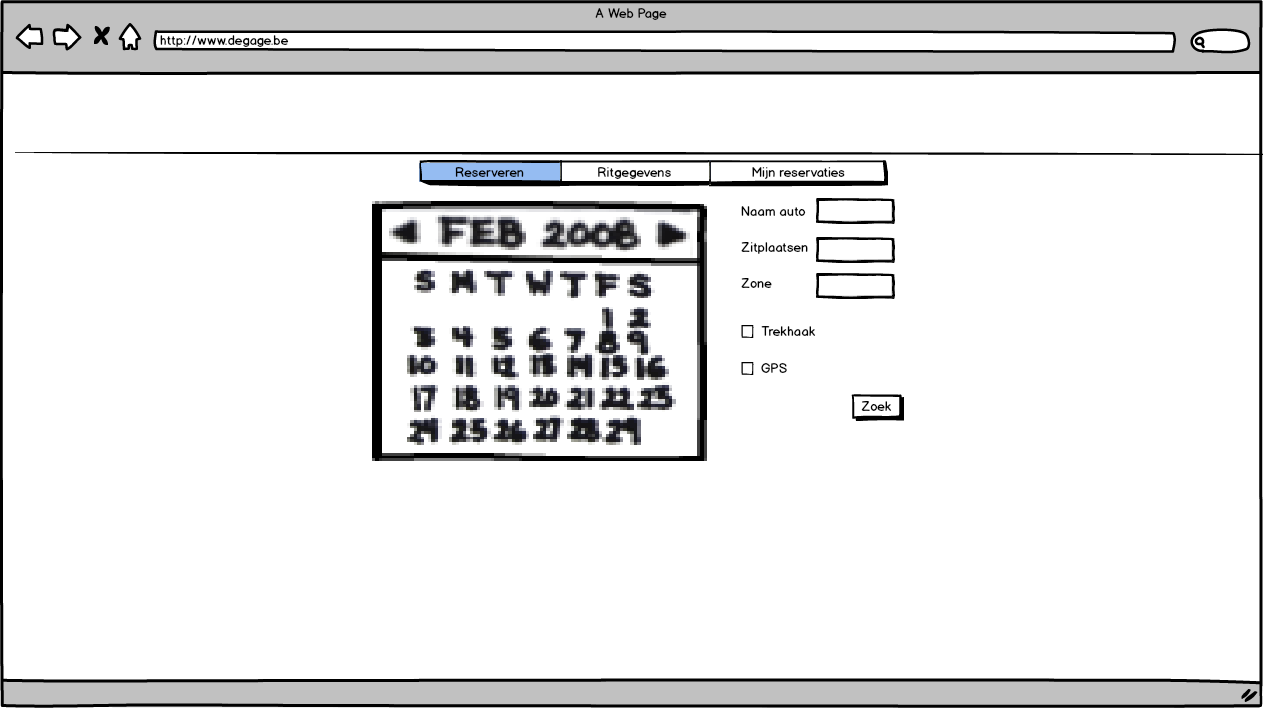
\includegraphics[width=\textwidth]{../../mockups/delen_reserveren.png}\end{figure}

\end{document}